
\section{Introduction}

In algebra, the solution to an equation is a number (or numbers), but the solution to a differential equations is a function (or functions). We will only be dealing with \textbf{ordinary differential equations} (ODEs) whose solutions are functions of only one variable. Believe it or not, you have seen a differential equation already! The anti-derivative
$$\int f(x)\ dx = F(x)+C$$
could be rewritten as the ODE
$$y' = f(x)$$
whose solution set is the family of functions $y=F(x)+C$. Of course, this means that differential equations can be more difficult to solve than antiderivatives, but this should give you this intuition of why differential equations can have a family of solutions. However, much like antiderivatives, if you specify an ``initial condition,'' a single solution for a differential equation can be determined. Here is a short example of a differential equation and its solution:
\begin{itemize}
\item The differential equation
$$y' + y = 2x$$
has solution 
$$y(x) = C e^{-x} + 2 x - 2$$
for any $C$, since
$$
\left[C e^{-x} + 2 x - 2\right]'+\left(C e^{-x} + 2 x - 2\right)=
-C e^{-x} + 2+ C e^{-x} + 2 x - 2 = 2x.
$$
Now if we specify the initial condition $y(0)=1$, we get
$$ 1=y(0)=C e^{-0} + 2 (0) - 2 = C - 2,$$
so $C=3$.
\end{itemize}

In the rest of this section you will learn techniques for solving two types of ODEs (separable and second order), and you will learn a way to approximate solutions (Euler's method). Afterwards, you will see some specific differential equations and their relation to different areas in science.


\section{Slope Fields and Euler's Method}

Some differential equations are of the form 
$$y'=f(x,y).$$
In this case, we can draw a \textbf{slope field}, where at each point $(x,y)$ we draw a line segment whose slope is $f(x,y)$. 

\begin{figure}[H]
\centering
\fbox{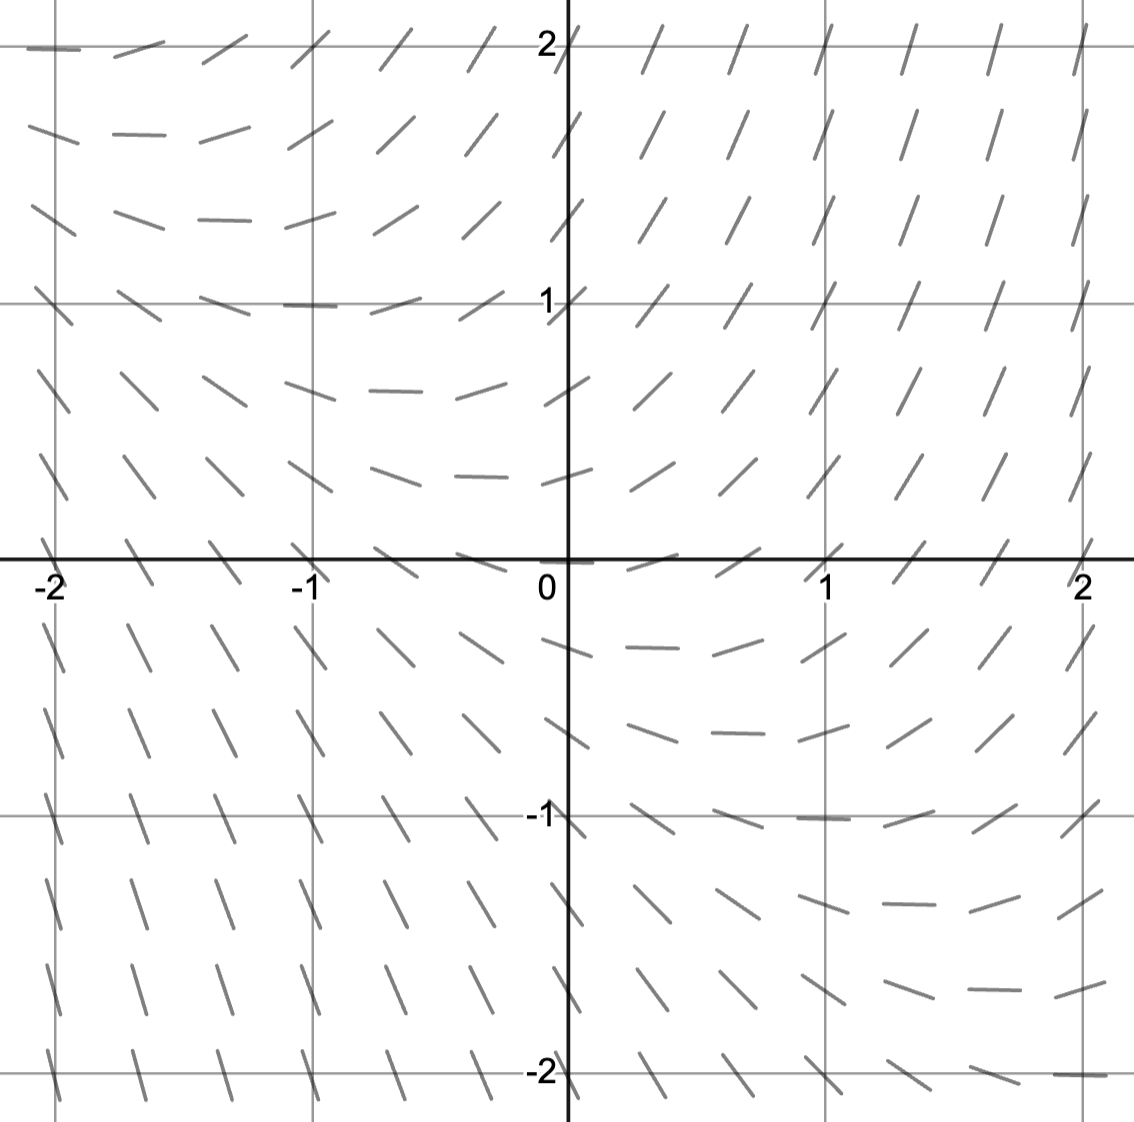
\includegraphics[width=3in]{img/slope_field.png}}
\caption{The slope field $y'=x+y$.}
\end{figure}

\mar{Draw the slope field for $y'=x-y$.}

Imagine a slope field to be a pool of water where the line segments show the current of water at each point. Then if you drop a ping pong ball somewhere on the slope field, the curve traced by the trajectory of the ball will be a solution to the ODE $y'=f(x,y)$. \textbf{Euler's method} is a technique for estimating solutions to this type of ODE using this ``riding the wave'' analogy.


The main idea in Euler's method is to use the slope at a point to determine a direction to move, and move a little bit in that direction. Now you're at a new point, so you repeat this process. The less you move each time, the closer the approximation will be to the actual solution.

In general, to do Euler's method you need to pick a step size for the $x$ direction: $\Delta x$. Then if you start at the point $(x_0, y_0)$, the next point will be
$$(x_1,y_1) = (x_0 + \Delta x, y_0 + \Delta y),$$
Where $\Delta y = \Delta x\cdot f(x_0, y_0)$. This formula comes from using the line at $(x_0, y_0)$ with slope $f(x_0, y_0)$. \mar{Do the algebra to see this.} The step size should be as small as possible for the approximation to be good, but in practice you will most likely use $1$, $\frac12$, $\frac1{10}$, or something else easy for computation. Here is an example:
\begin{itemize}[leftmargin=1em]
\item For the ODE $y'=x+y$, we'll do Euler's method with $\Delta x = 1$, and then again with $\Delta x = \frac{1}{2}$. For both we'll use $(x_0,y_0)=(-1,2)$. The easiest way to do these computations is in a table, computing row by row, using the $\Delta y$ in the previous row to increment to the next value of $y$.

\begin{multicols}{2}
\begin{center}
\def\arraystretch{1.2}
\begin{tabular}{@{}cccc@{}}
\multicolumn{4}{c}{$\Delta x = 1$}\\
\midrule[0.4mm]
$x$ & $y$ & $f(x,y)$ & $\Delta y = \Delta x f(x,y)$ \\
\midrule
$-1$ & $1$ & $0$ & $0$\\
$0$ & $1$ & $1$ & $1$\\
$1$ & $2$ & $3$ & $3$\\
$2$ & $5$ & $7$ & $7$\\
$3$ & $12$ & $15$ & $15$\\
\bottomrule[0.4mm]
\end{tabular}
\end{center}

\columnbreak

\begin{center}
\def\arraystretch{1.2}
\begin{tabular}{@{}cccc@{}}
\multicolumn{4}{c}{$\Delta x = 1/2$}\\
\midrule[0.4mm]
$x$ & $y$ & $f(x,y)$ & $\Delta y$ \\
\midrule
$-1$ & $1$ & $0$ & $0$\\
$-1/2$ & $1$ & $3/2$ & $3/4$\\
$0$ & $7/4$ & $7/4$ & $7/8$\\
$1/2$ & $7/4$ & $9/4$ & $9/8$\\
$1$ & $23/8$ & $31/8$ & $31/16$\\
\bottomrule[0.4mm]
\end{tabular}
\end{center}
\end{multicols}

\mar{Make a table for $\Delta x = 1/4$ and graph the points.}
Here is a graph of the points in these two tables ($\Delta x = 1$ in red and $\Delta x = 1/2$ in blue). In addition, the actual solution to this ODE ($y=e^{x+1}-(x+1)$) is graphed in black.
\begin{center}
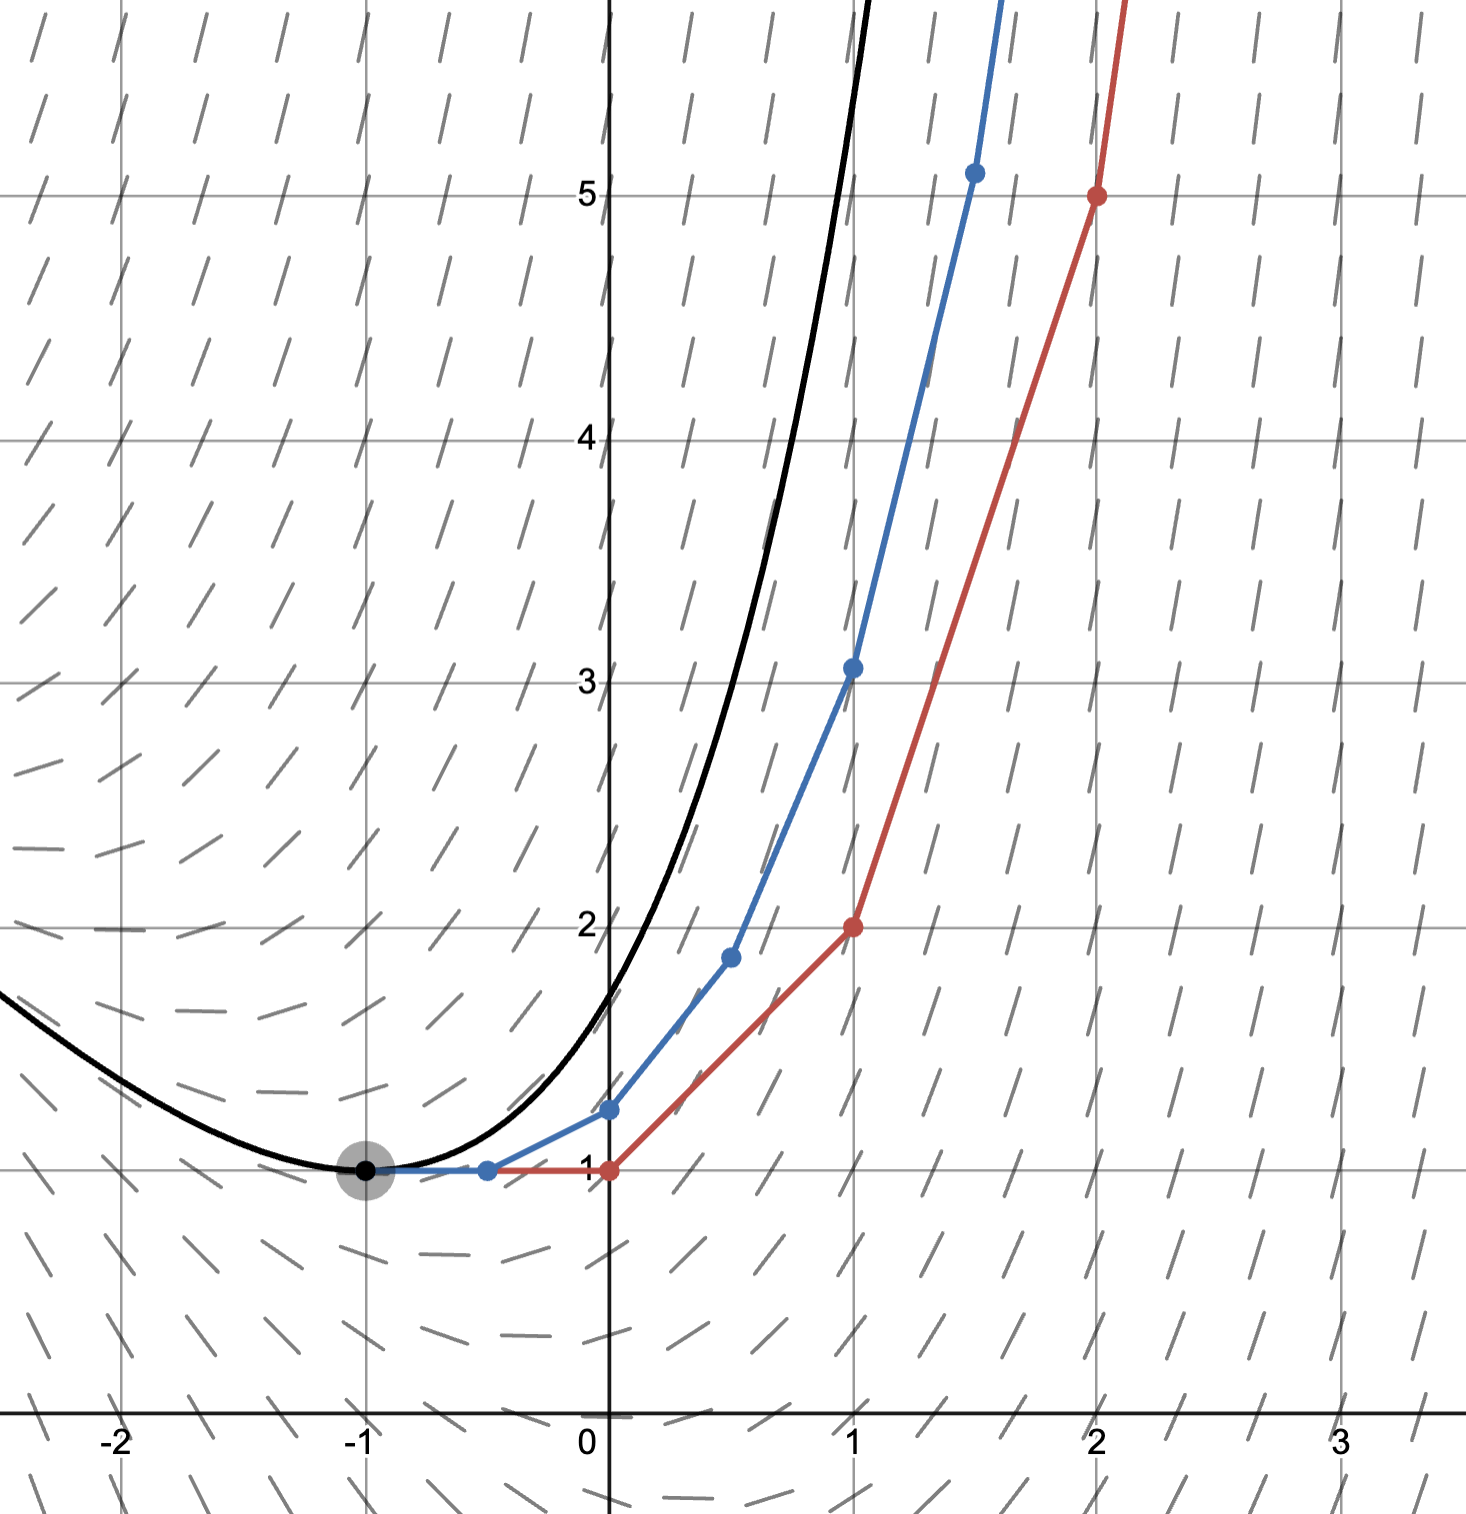
\includegraphics[width=3in]{img/eulers_method.png}
\end{center}
As you can see, the smaller step size gave a better approximation.
\end{itemize}


\section{Solving ODEs}
\subsection{Separable ODEs}
The first kind of ODE that you can solve by hand is on expressible as one or two integrals by \textit{separating} the $x$ and $y$ variables. These are of the form
$$y'=f(x)g(y) \quad\quad\text{or}\quad\quad \frac{dy}{dx}=f(x)g(y)$$
and can be rewritten as
$$\frac{1}{g(y)}\ dy = f(x)\ dx.$$
Both sides of this equation can be differentiated (the left with respect to $y$ and the right with respect to $x$). The resulting equation is the solution. Here is an example:
\begin{itemize}
\item For the ODE $\frac{dy}{dx} = xy$, rewrite as
$$\frac{1}{y}\ dy = x\ dx.$$
Integrating both sides gives
$$\ln|y| = \frac{x^2}{2} + C.$$\mar{Why is it ok that there is a constant only on one side?}
Thus for any $C$, the curve defined be the equation above is a solution. You do not need to solve for $y$.
\end{itemize}

\subsection{Second Order Differential Equations}

The next type of differential equation we can solve by hand is a \textbf{second order homogeneous linear differential equation with constant coefficients}, which has general form
$$ay''+by'+c=0$$
where $a$, $b$, and $c$ are real numbers. It is called \textbf{homogeneous} since the right hand side is 0 (there are no terms with an $x$) and it is linear since each term is a real number times a derivative of $y$. 

If $a=0$, then the ODE is separable and you can solve it by the technique described in the previous section. If $a$ is not 0, the solutions to this ODE will be exponential and depend on the roots of the polynomial
$$a\lambda^2 + b\lambda + c = 0,$$
which is called the \textbf{characteristic equation}.
This is because plugging $y=e^{\lambda x}$ into the ODE and dividing by $e^{\lambda x}$ gives this equation. \mar{Plug $y=e^{\lambda x}$ into the ODE and get this quadratic equation.} The root(s) in question are
$$\lambda = \frac{-b \pm \sqrt{b^2-4ac}}{2a}.$$
 There are two cases:
\begin{enumerate}
\item The discriminant $b^2-4ac$ is nonzero. In this case, there are two roots $\lambda_1$ and $\lambda_2$. Then the solutions are of the form
$$y=pe^{\lambda_1 x} + qe^{\lambda_2 x},$$
for any real numbers $p$ and $q$. Keep in mind that if $b^2-4c$ is negative, then $\lambda_1$ and $\lambda_2$ will be imaginary (see the appendix on complex numbers). \mar{What is a way to write $e^{(a+bi)x}$ without a complex number in the exponent?}
\item The discriminant $b^2-4c$ is zero. In this case, the only root is $\lambda = -b/2$. Then the solutions are of the form
$$y=pe^{\lambda x}+qxe^{\lambda x}$$
for any real numbers $p$ and $q$.
\end{enumerate}

An interesting and useful fact is given in this theorem:
\begin{thm}
If $y_1$ and $y_2$ are solutions to a homogeneous ODE then so is the linear combination $p{y_1}+q{y_2}$ for any real $p$ and $q$.
\end{thm}
 
Sometimes it is considered ``good form'' to express solutions to an ODE using only real numbers. If that is desired, use this theorem to take linear combinations of solutions you have to generate those with only real numbers.

\section{Applications}
\subsection{The Logistic Equation}
\subsection{Simple Harmonic Oscillator}
\subsection{Predator-Prey}
